\chapter{La via Lattea}
La \emph{Via Lattea} \`e la galassia in cui noi abitiamo. Il sistema solare \`e posizionato in uno dei suoi bracci in una zona molto periferica. Classificandola in modo pi\`u tecnico, si tratta di una galassia \emph{spirale barrata}\footnote{Nome che indica come sono disposta le braccia della galassia}. Pu\`o essere suddivisa in alcuni zone principali che prendono il nome di
\begin{center}
\begin{tabular}{c c c c}
	\hline
	\hline
	Zona & Massa & R & Geometria \\
	\hline
	\hline
	Alone Stellare & $10^9M_{\odot}$ & $r\sim20kpc$ & Sferico\\
	Disco di Gas   & $10^{10}M_{\odot}$ & $r\sim25kpc$ & Disco $h=0.15kpc$\\
	Rigonfiamento Centrale & $10^{10}M_{\odot}$ & $(6\times2\times2)Kpc$ & Ellissoide\\
	Disco Stellare & $10^{11}M_{\odot}$ & $r\sim15kpc$ & Disco $h=1kpc$\\
	Alone Dark Matter & $10^{12}M_{\odot}$ & $r>60kpc?$ & Sferico\\
	\hline
\end{tabular}
\end{center}
Le stelle nella galassia sono organizzate in \emph{ammassi} che possono essere di due tipi: \emph{Ammassi Globulari} e \emph{Ammassi Aperti}. Gli ammassi globulari sono distribuiti nell'alone galattico, mentre gli ammassi aperti sono situati nel disco stellare. Le principali caratteristiche di entrambi sono riassumibili in
\begin{center}
\begin{tabular}{c c c c c c}
	\hline
	\hline
	Ammasso & $N^o$ Stelle & Dimensioni & Gas & Neb. Planetarie & $N^o$ Conosciuti \\
	\hline
	\hline
	Aperto & $10^3$ - $10^4$ & $10pc$ & S\`i & No & $10^3$\\
	Globulare & $10^4$ - $10^6$ & $(20$ - $100)pc$ & No & S\`i & 160\\
	\hline
\end{tabular}
\end{center}
\section{Dinamica degli Ammassi Globulari}
Gli ammassi globulari, essendo sistemi composti da molte stelle, viene spontaneo tentare di applicare i metodi della termodinamica per studiarne la dinamica. Non \`e possibile per\`o trattare l'ammasso globulare come un gas perfetto. La teoria di gas perfetto \`e una teoria non-interagente, mentre in questo caso si hanno interazioni stella-stella ed \`e di tipo a \emph{lungo-range}. Questo complica lo studio delle traiettorie delle singole particelle. Si adotta un approccio di tipo campo medio usando il \emph{teorema del viriale} che in questo caso si pu\`o applicare in quanto si ha a che
\begin{itemize}
	\item Particelle che si muovono in uno spazio limitato $V$.
	\item $G=\sum_{i=1}^Nr_ip_i$\`e una quantit\`a finita. 
	\item $G\to cost$.
\end{itemize}

Per la limitatezza di $G$ si ha che 
\newl{\abs{G} = \abs{\sum_{i=1}^N r_i p_i} \leq \left. \sum_{i=1}^N\abs{r_i} \cdot \abs{p_i} \right|_{V} \leq NR_vP}
dove $R_v$ \`e stato ipotizzato limitato, quindi $G$ \`e limitata. Pi\`u o meno nello stesso modo \`e possibile mostrare il comportamento di $G$ per $t\to+\infty$
\newl{
	\abs{\left\langle\frac{d}{dt}G \right\rangle} = \abs{\lim_{\tau\to+\infty}\frac{1}{\tau}\int_{0}^{\tau}\frac{d}{dt}G\, dt } = \abs{\lim_{\tau\to\infty}\frac{G(\tau)-G(0)}{\tau}} \leq \abs{\lim_{\tau\to+\infty} \frac{2NR_vP}{\tau} } = 0
}
quindi per $t\to+\infty$, $G$ tende ad una costante. A questo punto \`e possibile enunciare che \emph{Il viriale, dopo un certo tempo di rilassamento, \`e costante}. Partendo dall'enunciato si dedurranno tutte le propriet\`a principali del viriale.

\newtheorem*{mydef}{Enunciato del Viriale}
\begin{mydef}
	\newl{ \left\langle k_t \right\rangle = -\frac{1}{2}\left\langle \sum_{i=1}^N r_i\cdot F_i \right\rangle_t \text{ Dove } k_t = \sum_i^N k_i \text{ energia cinetica totale} \label{enun:vir}}
\end{mydef}

\begin{proof}[Dimostrazione]
Partendo dal risultato ottenuto precedentemente sulla derivata di $\left\langle G' \right\rangle=0$ \`e possibile scrivere
\newl{\left\langle \frac{d}{dt} \sum_{i=1}^Nr_i \cdot p_i \right\rangle = 0 }
facendo le derivate
\newl{\left\langle 2\sum_{i=1}^Nk_i + \sum_{i=1}^Nr_i\cdot F_i \right\rangle = 0 \nonumber\\
	\left\langle k_t \right\rangle = -\frac{1}{2}\left\langle \sum_{i=1}^N r_i\cdot F_i \right\rangle }
\end{proof}
Questo per un caso generale. Considerando il caso specifico di forze centrali si il \emph{Teorema del Viriale per Forze Centrali}.
\newtheorem*{mydef2}{Viriale per forze centrali}
\begin{mydef2}
Il teorema del viriale per un campo di forze centrali del tipo 
\newl{U(r)\sim \frac{1}{r^{\alpha}},}
si scrive nella forma
\newl{ \left\langle K \right\rangle = -\frac{\alpha}{2}\left\langle U \right\rangle_t .}
Nel caso specifico della forza di attrazione gravitazionala si ha che $\alpha=1$.
\end{mydef2}
\begin{proof}
Per dimostrarlo si parte dall'enunciato del viriale dato precedentemente in cui si sostituisce la forza di interazione gravitazione tra $N$ particelle. Sapendo quindi che
\newl{F_{i,j} = k \frac{r_i - r_j}{\abs{r_i-r_j} ^3 } , }
in particolar modo, la forza su una singola particella \`e pari a
\newl{F_i = \sum_{j=1,j\neq i}^N F_{i,j} = k \sum_{j=1,j\neq i} \frac{r_i - r_j}{\abs{r_i-r_j} ^3 } }
e sostituendo in Eq.~\ref{enun:vir} si ottiene
\newl{-\frac{1}{2} k \left\langle \sum_{i=1}^N\left( r_i  \sum_{j=1,j\neq i} \frac{r_i - r_j}{\abs{r_i-r_j} ^3 }\right)   \right\rangle = -\frac{1}{2} k \left\langle \sum_{i=1}^N \sum_{j=1,j\neq i} \frac{r_i\left(r_i - r_j\right)}{\abs{r_i-r_j} ^3 }   \right\rangle = \nonumber \\
	= -\frac{k}{2}\sum_{i=1}^N \sum_{j\neq i}^N \left( \frac{(r_i-r_j)^2}{\abs{r_i-r_j} ^3} +\cancel{ \frac{(r_i-r_j)(r_i+r_j)}{\abs{r_i-r_j} ^3}} \right)= -\frac{1}{2}\sum_{i=1}^N \sum_{j\neq i}^N \frac{k}{\abs{r_i-r_j} } = \nonumber\\ 
	= -\frac{1}{2} 2U = -\frac{1}{2}U.
}
\end{proof}
Usando il teorema del viriale con gli ammassi globulari \`e possibile fare stimare molte grandezze fisiche. Per avere degli ordini di grandezze che siano un minimo attendibili si consideri un ammasso globulare standard composto da $10^6$ stelle e di raggio $R=5pc$. Con questi valori \`e possibile calcolare
\begin{itemize}
	\item Energia potenziale dell'ammasso $U$;
	\item Componente media cinetica $K$;
	\item Velocita` quadratica media $\left\langle v^2 \right\rangle$;
	\item velocit\`a di fuga $v_{fuga}$;
	\item Tempo di rilassamento $T_rel$;
	\item Massa totale dell'ammasso $M$;
\end{itemize}
\newtheorem*{mydef3}{Calcolo energia potenziale}
\begin{mydef3}
\newl{U = -\frac{3}{5} \frac{GM^2}{R} = -2.5\cdot 10^{51} erg  }
\end{mydef3}

\newtheorem*{mydef4}{Calcolo componente cinetica media}
\begin{mydef4}
Sapendo $U$ posso calcolare la componente cinetica media usando il teorema del viriale
\newl{\left\langle K \right\rangle_t = -\frac{1}{2} \left\langle U \right\rangle = - 1.2\cdot 10^{51} erg}
\end{mydef4}
Da notare che l'energia totale del sistema \`e minore di zero, questo implica che il sistema \`e legato e stabile, quindi \`e ormai termalizzato.

\newtheorem*{mydef5}{Velocit\`a quadratica media}
\begin{mydef5}
	\newl{\frac{1}{2} M_{*} \cdot N \cdot \frac{1}{N}\sum_{i=1}^N v_i^2 = \frac{1}{2}M_{tot}v_{m}^2\nonumber \\
	v_m = \sqrt{\frac{3GM_{tot}}{5R}} = 16 km/s   }
\end{mydef5}

\newtheorem*{mydef6}{Velocit\`a di fuga}
\begin{mydef6}
	\newl{\frac{1}{2}M_{*} v_f^2 - G\frac{M_{*} M_{tot}}{R} = 0 \nonumber\\
		v_f=\sqrt{\frac{2GM_{tot}}{R}} = 29 km/s
	}
\end{mydef6}
Il fatto che $v_m < v_f$ \`e a riprova di quello ricavato nel calcolo dell'energia totale dell'ammasso, cio\`e che \`e un sistema legato e stabile. Sia il calcolo totale dell'energia del sistema che il calcolo della velocit\`a media a confronto con quella di fuga, suggeriscono che gli ammassi globulari siano sistemi di stelle stabili, legati e quindi, usando un termine termodinamico", termalizzati. \`E quindi interessante scoprire il tempo che un ammasso globulare impega per termalizzare. A questo scopo i prossimi calcoli saranno concentrati sul trovare un modello esaustivo di interazioni che spieghi il modo in cui questi ammassi stellari termalizzano. Il tempo che un ammasso stellare impiega per entrare in una condizione di stabilit\`a viene definito \emph{Tempo di Rilassamento}.

\newtheorem*{mydef7}{Determinazione del Tempo di Rilassamento}
\begin{mydef7}
	Dato che gli ammassi globulari sono realt\`a stabili, il tempo di rilassamento deve essere almeno inferiore all'et\`a dell'universo.
\end{mydef7}
Per determinare il tempo di rilassamento dell'ammasso \`e necessario dare una definizione appropriata di \emph{ammasso rilassato}. Una prima definizione che \`e possibile dare consiste nel dire che l'ammasso, formato da $N$ stelle, \`e rilassato dopo che ogni stella che lo costituisce ha fatto $N$ interazioni con le altre.

Da questa definizione segue la necessit\`a di definire quando c'\`e interazione tra due stelle. 
Il primo tentativo di descrivere l'interazione \`e attraverso un raggio di cut-off che chiameremo \emph{Raggio di Collisione}, cio\`e la distanza massima per far si che due stelle formino uno stato legato. In questo modo la definizione di raggio di collisione viene spontanea
\newl{\frac{1}{2}M_{*}v^2 = G\frac{M_{*}}{r_c}, \nonumber\\
	r_c = 2 \frac{GM_{*}}{v^2}.
}
Ora \`e necessario definire una probabilit\`a di interazione tra le stelle. Questa dipender\`a dalla velocit\`a della stella e dalla densit\`a dell'ammasso. Sia $n$ la densit\`a stellare dell'ammasso, questo vuol dire che in un volume finito di dimensione $V=\pi r^2 \Delta x$ ci sono $N_{*}=n(\pi r^2 \Delta x)$ stelle, quindi una stella che attraversa questo volume dell'ammasso globulare compie al pi\`u un numero di interazioni pari a $N_{int} = N_{*}$. Riscrivendo meglio il volume in funzione anche della velocit\`a si ottiene che
\newl{(\pi r^2 v \Delta t)n = N_{int} \implicaa \Delta t = \frac{N_{int}}{n \pi r^2 v}.}
Usando subito la definizione di raggio di collisione si ottiene
\newl{\Delta t = \frac{N_{int} v^3 }{4\pi G^2 M_{*}^2  n}, }
ma $N_{int} \sim 1$ iunterazione ad una stella. Usando la definizione della densit\`a stellare e la definizione di $G$ uscente dal viriale
\newl{n=\frac{N}{\frac{4}{3}\pi R^3}\,\,\,\,\,\,\, G = \frac{R v^2}{M_{*}N}}
e supponendo che $3/5 \sim 1/2$ si ottiene la scrittura finale per $\Delta t$
\newl{\Delta t \sim \frac{NR}{3v}.}
Inserendo i valori tipici di un ammasso globulare si ottiene un tempo rilassamento medio di
\newl{\Delta t \sim \frac{1}{3} \frac{10^6 \times 5pc}{16 km / s} \sim 100 Gyrs }
che \`e un risultato fisicamente sbagliato. Come osservato precedentemente, gli ammassi globulari sono sistemi legati, quindi termalizzati. Questo suggerisce che nella stima di $\Delta t$ sono state fatte approssimazioni troppo forti che hanno reso il modello inattendibile. L'approssimazione pi\`u forte che \`e stata fatta riguarda la definizione di \emph{interaione tra le stelle}. \`E stato considerato che una stella interagisce con un'altra stella solo al di sotto del suo \emph{raggio di collisione}. In questo modo \`e stato messo un cut-off all'interazione facendola diventare a corto range. Naturalmente l'interazione gravitazionale \`e tipo \emph{a lungo range} quindi il passo successivo \`e quello di estendere l'interazione considerandola a lungo range e ricalcolare il tempo di rilassamento.
\begin{figure}
		\centering
		\fbox{
		\begin{tikzpicture}[scale=2,auto=center]
				\draw [->] (0,0) -- (4,0);
				\node[] at (0.3,0.6) {$*$};
				\node[] at (1,1) {$*$};
				\node[] at (1.3,0.2) {$*$};
				\node[] at (1.6,-0.7) {$*$};
				\node[] at (1.9,-0.3) {$*$};
				\node[] at (2.2,0.5) {$*$};
				\node[] at (2.5,0.9) {$*$};
				\node[] at (2.9,0.3) {$*$};
				\node[] at (3.3,-0.3) {$*$};
				\node[] at (3.6,-0.5) {$*$};
				\node[] at (3.9,-1) {$*$};
				
				\node[] at (0.3,-0.6) {$*$};
				\node[] at (1,-1) {$*$};
				\node[] at (1.3,-0.2) {$*$};
				\node[] at (1.6,0.7) {$*$};
				\node[] at (1.9,0.3) {$*$};
				\node[] at (2.2,-0.5) {$*$};
				\node[] at (2.5,-0.9) {$*$};
				\node[] at (2.9,-0.3) {$*$};
				\node[] at (3.3,0.3) {$*$};
				\node[] at (3.6,0.5) {$*$};
				\node[] at (3.9,1) {$*$};

				\node[] at (5,0.1) {$v$ corto-range};

				\draw[color=red,->] plot [smooth] coordinates {(0,0) (1,0.3) (2,-0.4) (3,0.5) (4,0.3) };

				\node[color=red] at (5,0.5) {$v$ long-range};

				\draw[->] (1,0.3) -- (1,0);
				\draw[->] (2,-0.4) -- (2,0);
				\draw[->] (3,0.5) -- (3,0);
				\draw[->] (4,0.3) -- (4,0);

				\node[] at (3.25,0.2) {$\Delta v_{\perp}$};
	
		\end{tikzpicture}
		}
		\caption{Andamento della velocit\`a della stella di riferimento nell'ammasso globulare nei due diversi modelli: interazione a corto-range ed interazione a lungo-range}
\end{figure}

Il punto di questo approccio consiste nel valutare i vari $\Delta v_{\perp}$ dalla direzione iniziale considerando l'interazione a corto range. La distribuzione delle stelle \`e possibile considerarla random quindi $\left\langle\Delta v_{\perp}\right\rangle=0$, la grandezza che pu\`o dare informazioni interessanti \`e $\left\langle\Delta v_{\perp}^2\right\rangle$, perch\`e \`e legato all'energia che la stella acquista, aumenta nel tempo e diventa significativamente importante per $\left\langle\Delta v_{\perp}^2\right\rangle \sim v^2$. 
\begin{figure}
		\centering
		\fbox{
		\begin{tikzpicture}[scale=1.3,auto=center]
				\draw[->] (-0.6,0) -- (0.4,0); 
				\draw[dashed,->] (2,0) arc (270:360:2);
				\draw[->] (4,3) -- (4,4);
				\node[] at (-1.1,0) {MRU};
				\node[] at (4.7,3.8) {MRU};
				\node[] at (4.1,0.6) {MCU};
				\node[] at (0.5,0) {$*$};
				\node[] at (2,2) {$*$};
				\node[] at (4,4.1) {$*$};

		\end{tikzpicture}
		}
		\caption{Tipo di interazione per $r>r_c$}
\end{figure}

Caratterizzata l'interazione per $r>r_c$ come
\newl{
		M_{*} \frac{\Delta v_{\perp}}{\Delta t} = G\frac{M_{*}^2}{r^2}\nonumber \\
		\Delta v_{\perp} = G\frac{M_{*}}{rv}
}
da cui \`e possibile valutare $\left\langle\Delta v_{\perp}^2\right\rangle$ facendo una media pesata sui
\newl{
		\left\langle\Delta v_{\perp}^2\right\rangle = \int_{r_c}^R \left(2\pi r dr\right)\left(v\Delta t \right)n\left(\frac{GM_{*}}{rv}\right)^2 =  \frac{2\pi n G^2 M_{*}}{v} \Delta t \log\left(\frac{R}{r_c}\right) = \nonumber \\
		= \frac{2\pi n G^2 M_{*}}{v} \Delta t \log\left(\frac{R v^2}{G M_{*}}\right) \sim \frac{2\pi n G^2 M_{*}}{v} \Delta t \log\left(N\right) 
}
valuto ora il $\Delta t$ tale che il contributo di $\left\langle\Delta v_{\perp}^2\right\rangle\sim v^2$ quindi
\newl{
		\Delta t = \frac{v^3}{2\pi n G^2 M_{*}^2 \log(N)} \sim \frac{1}{12 \ln(N/2)} \frac{N R}{v} \sim 2 Gyrs < ETA_{universo}
}
quindi per un ammasso globulare tipico si ha un tempo tipico di rilassamento di circa $2Gyr$, risultato compatibile con le osservazioni precedenti. Per stimare l'et\`a di un ammasso globulare ci sono altri metodi quali turn-off point e attraverso la stima della \emph{Luminosity Function}.
\section{Ammassi Aperti}
Una seconda classe di ammassi presenti nella Via Lattea sono gli \emph{Ammassi Aperti}. Sono situati sul disco galattico e sono formati da stelle e solitamente anche da gas e polveri.

La popolazione stellare degli ammassi aperti arriva da statistiche fatta su circa $1000$ ammassi aperti censiti entro i $2kpc$ dalla terra. \`E difficile osservare ammassi aperti pi\`u distanti a causa delle polveri del disco galattico. Questo implica il fatto che il numero di ammassi aperti galattici che conosciamo oggi sono una forte sottostima, ma comunque permette di concludere ugualmente che la popolazione degli AA \`e molto pi\`u numeorsa di quella degli AG.
\begin{figure}
		\centering
		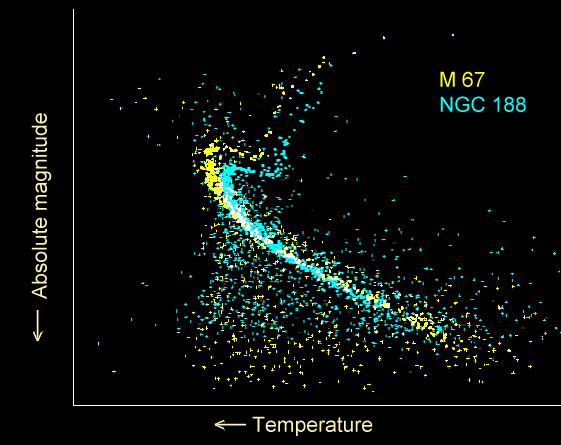
\includegraphics[scale=0.4]{turnM67.png}
		\caption{Diagramma HR di M67 e NGC188 messi a confronto. Il diverso punto in cui avviene il Turn-off indica l'et\`a diversa dell'ammasso}
		\label{ETA:AA}
\end{figure}

In Fig.~\ref{ETA:AA} \`e presentato il diagramma HR della popolazione di stelle di due diversi ammassi aperti. Valutando la posizione del \emph{turn-off} point \`e possibile stimare l'et\`a dell'ammasso. Con lo stesso ragionamento utilizzato in precedenza per gli ammassi globulari possiamo stimare il tempo di rilassamento anche degli ammassi aperti come
\newl{\Delta t_r \sim \frac{\sqrt{NR^3}}{12\log(N/2)\sqrt{GM_{*}}} \sim 10^9Gyr}
che indica in modo evidente che la gran parte degli ammassi aperti che si conoscono non \`e rilassata.
Gli ammassi aperti hanno et\`a molto giovane perch\`e essendo situati all'interno del disco stellare hanno una probabilit\`a abbastanza alta di interagire con oggetti particolarmente massivi che possono letteralmente distruggere l'ammasso e in generale non hanno massa sufficiente per evitare l'evaporazione. Grazie alla rotazione differenziale del piano galattico l'ammasso aperto pu\`o entrare in stretta interazione con oggetti particolarmente massivi e quindi venir distrutti dalle varie \emph{forze mareali} a cui sono sottoposti.
\section{Il Mezzo Interstellare}
















